\section{Estruturação da \textit{String} de Busca}

Para estruturar a delimitação da busca na base digital, utilizou-se o protocolo PICO, proposto na área da medicina. Procederam-se as adaptações necessárias para o contexto da engenharia de \textit{software}. PICO é um acrônimo para \textit{patient} (população de pacientes), \textit{intervention} (intervenção), \textit{comparison} (comparação) e \textit{outcome} (resultado) e pode ser representado como um gráfico de \textit{Venn}, como observado na figura \ref{fig:pico} \cite{pai_clinical_2004}.




\begin{figure}
    \centering
    \caption{Representação Visual do Protocolo PICO }
    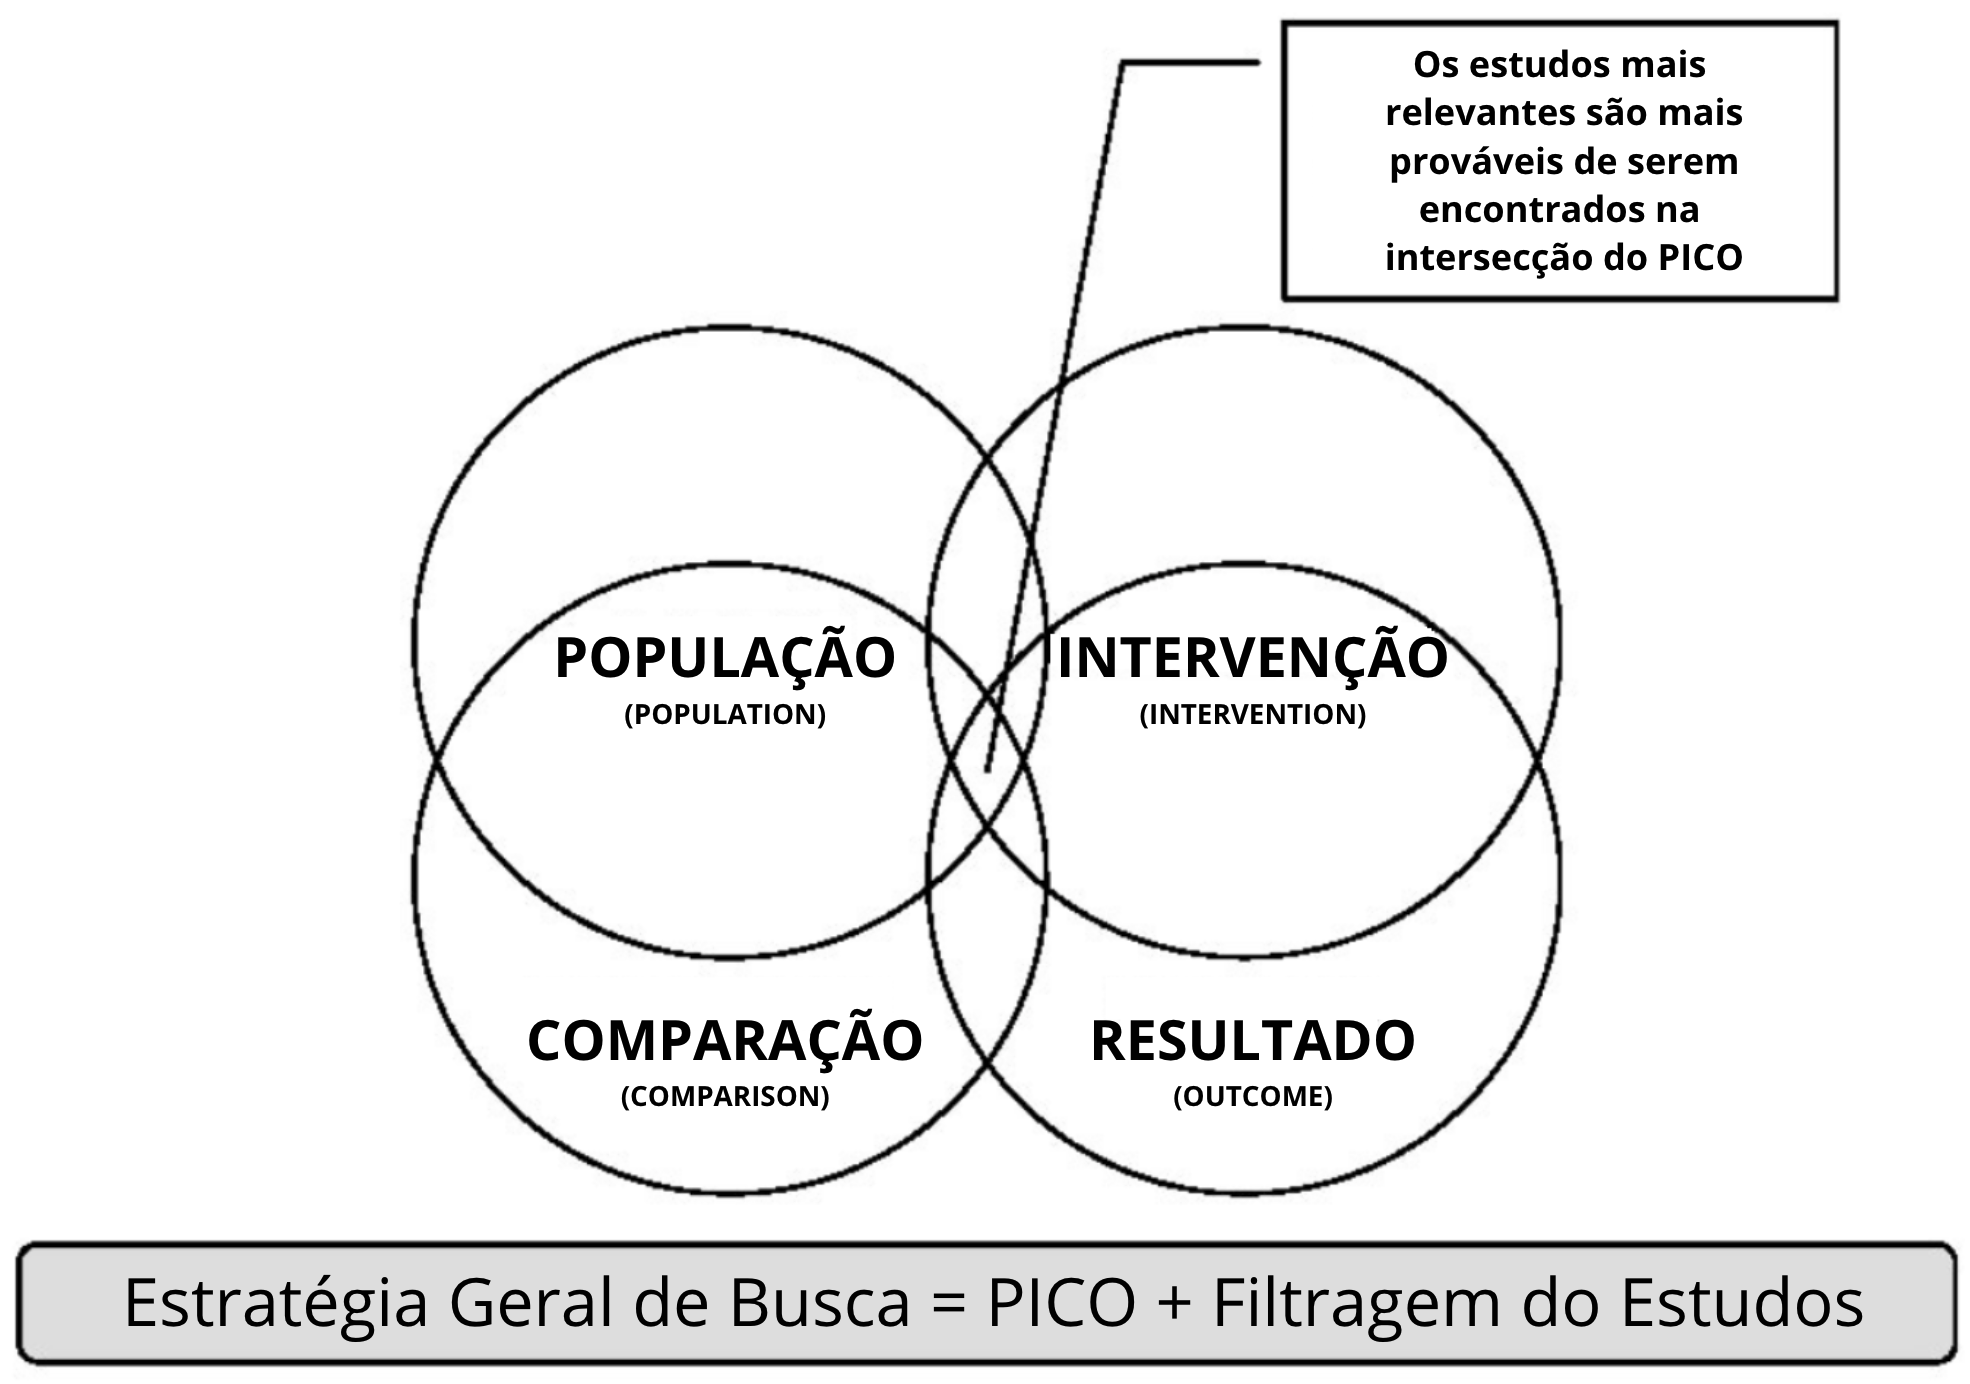
\includegraphics[width=0.75\linewidth]{figuras/PICO.png}
    \text{Fonte: Adaptado de \citeonline{pai_clinical_2004}}
    \label{fig:pico}
\end{figure}

Considerando o contexto do produto investigado nesta monografia, a \textbf{população de pacientes} equivale a sua área específica da engenharia de software, o desenvolvimento \textit{web}. Na medicina, a \textbf{intervenção} se refere ao tratamento a ser aplicado e analisado, então, foram utilizados termos relacionados a experimentação contínua. O \textbf{resultado} representa a saída relatada nos estudos a serem selecionados e, em busca de compreender o estado da arte, foram adicionados termos que representassem estudos secundários e terciários, como revisão da literatura, mapeamento sistemático, etc. Já a \textbf{comparação} seria a adição de outros tipos de intervenção a serem comparadas com a principal. Porém, dado que a área da Engenharia de \textit{Software} ainda é muito nova, o corpo de conhecimento ainda não é tão bem organizado como na medicina, o que impede que esta camada da \textit{string} funcione como proposto na área médica, por isso, não foi utilizada.

Desta forma, os termos utilizados foram gerados a partir da união da \textit{string} de busca do estudo de controle e das expressões que o mesmo trouxe como utilizadas na literatura para se referir à experimentação contínua e tópicos relacionados. A estrutura consolidada é apresentada na Tabela \ref{tab:string-busca}.


\begin{table}[]
\caption{Estrutura dos Termos da String de Busca}
    \begin{tabular}{|p{2cm}|p{3cm}|p{9cm}|}
        \hline
        \textbf{Camada} & \textbf{Palavra Chave} & \textbf{Sinônimos} \\ \hline
        População & \textit{software development} & \textit{software engineering} 
         e \textit{web development} \\ \hline
        Intervenção & \textit{continuous experimentation} & \textit{continuous software experimentation}, \textit{experiment systems}, \textit{data-driven development}, \textit{A/B tests}, \textit{online controlled experiments}, \textit{innovation experiment system}, \textit{experiment-driven software development}, \textit{evidence-based software engineering}, \textit{experimentation system}, \textit{customer-driven development} e \textit{experiment-driven development} \\ \hline
        Resultado & \textit{systematic literature review} & \textit{secondary studies}, \textit{tertiary studies}, \textit{literature review} e \textit{systematic literature mapping} \\ \hline
    \end{tabular}

    \begin{center}
        \text{Fonte: Autor}
        
    \end{center}

\label{tab:string-busca}
\end{table}

Para finalizar, adicionou-se o operador lógico 'AND' para separar cada camada do protocolo e, dentro de cada uma delas, o operador lógico 'OR' para separar as palavras-chave e seus sinônimos. Acrescentou-se também sintaxes específicas da base de dados para realizar o truncamento de termos, a fim de abranger diferentes terminologias para as mesmas palavras chave. Isto resultou na string finalizada da seguinte forma:

\textit{("software development" OR "software engineering" OR "web development") 
AND 
("continuous experimentation" OR "continuous software experimentation" OR "experiment systems" OR "data-driven development" OR "A/B test*" OR "online controlled experiment*" OR "innovation experiment system" OR "experiment-driven software development" OR "evidence-based software engineering" OR "experimentation system" OR "customer-driven development" OR "experiment-driven *") 
AND 
("secondary stud*" OR "tertiary stud*" OR "literature review" OR "systematic literature review" OR "systematic literature mapping" OR "combined process") 
}